%Die Angabe des schlauen Spruchs auf diesem Wege funtioniert nur,
%wenn keine Änderung des Kapitels mittels den in preambel/chapterheads.tex
%vorgeschlagenen Möglichkeiten durchgeführt wurde.
\chapter{Experimental Setup}
\label{chap:chapter5}
%\vspace{-3cm}
%\vspace{2cm}
With the feature selection and their extraction explained in earlier chapter, we ca now move to the methodology for experiments. This chapter focuses on three topics - first, being the assumptions for the test setup and the configuration of the sample population as well as the method used to generate the sample population, explained in the section~\ref{sec:gsp}. Second, criteria for selection of the machine learning algorithm among those already surveyed in the chapter~\ref{chap:chapter3} is described in the section~\ref{sec:selml}. Third part, in the section~\ref{sec:mltools} briefly describes tools surveyed for using the selected machine learning algorithm.
\section{Generation of sample population}
\label{sec:gsp}
Sample population is required to train and cross-validate the machine learning based classifier (hereon referred simply as \emph{classifier}). A separate set of data is used to test the accuracy of the classifier.
\subsection{Assumptions}
\label{sec:gsp:assumptions}
Following are the assumptions while generating the sample population and test data:
\begin{enumerate}
  \item Sample population is generated per circuit type \emph{i.e.} all examples in sample population for a circuit type are generated by simulating a single netlist with different fault instances. 
  \item It is assumed that the chips to be classified have displayed faulty behavior and hence were rejected in earlier test.
  \item The chips under consideration are either:
		  \begin{enumerate}
    		\item Healthy chips with transient noise or
    		\item Affected by a single permanent or intermittent fault, with or without transient noise.
 		 \end{enumerate}
	\item Permanent faults are modeled using stuck-at, wired or delay faults, Intemittents are modeled using high frequency power droop, and transient faults are modeled as conditional stuck-at faults at random locations, triggered using deterministic fault rate.
	\item Number of simulation runs to extract features is fixed at 4. This value is set experimentally. 
\end{enumerate}

\subsection{Configuration}
For the purpose of running experiments uniformly on different circuit types, a sample population and a test set for each of cicuit types is created with following configuration:
\begin{enumerate}
  \item A sample population consist of 2500 ($\pm$ 75) of labeled examples. The tolerance of $\pm$ 75 is set as the permanent or intermittent fault instances which did not show any faulty behavior at POs at all were removed.
  \item The sample population is equally divided into following five fault categories:
		\begin{enumerate}
    		\item Permanent faults with label \texttt{P}.
    		\item Permanent faults along with transient noise (fault rate = 0.001) with label \texttt{P}.
			\item Intermittent faults (fault rate = 0.1, 0.01 0.001) with label \texttt{I}.
    		\item Intermittent faults (fault rate = 0.1, 0.01, 0.001) along with transient noise (fault rate = 0.001) with label \texttt{I}.
			\item Transient faults (fault rate = 0.01, 0.001, 0.0001) with label \texttt{T}.
 		 \end{enumerate}
  \item One-fourth of total population is separated out as cross-validation set, rest is used as training data.
  \item Test data has 250 ($\pm$ 15) labeled examples, with same configuration as that for sample population.
\end{enumerate}

\subsection{Implementation}

Sample population is generated as shown in figure~\ref{fig:sampopl} using a simulation framework called Adaptive Diagnosis of Arbitrary Manifold Artifacts (ADAMA). ADAMA can be used for logic simulation with error injection. Logical representation of a circuit at gate level and test pattern set are the required inputs for simulation using ADAMA. A fault description can be provided optionally to inject a fault and analyze its behavior. ADAMA supports all of the fault models that we have considered under our assumptions in section~\ref{sec:gsp:assumptions}.

\begin{figure}[h]
  \begin{center}
    \captionsetup{justification=centering}
    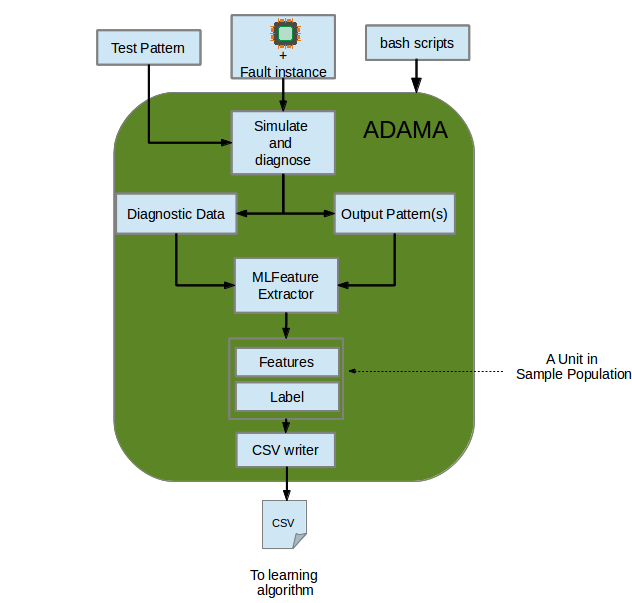
\includegraphics[scale=0.45]{figures/sampopl.png}
    \caption{Generation of sample population using \texttt{spgen}}
    \label{fig:sampopl}
  \end{center}
\end{figure}

For experiments, ADAMA framework has been extended by adding a task to generate sample population, called \texttt{spgen}.\texttt{spgen} takes fault description, circuit description and test pattern set as inputs along with number of simulations runs (\texttt{simruns}) to be performed for feature extraction. It then runs simulation and diagnosis \texttt{simruns} times and passes it on to the object of class \texttt{MLFeatureExtractor}, which encompasses all of the procedures for feature extraction described in section~\ref{sec:secfs} of previous chapter. Once complete simulation is over, it writes the features and its label in a CSV file.

Shell scripts are used to invoke instances of ADAMA and inject fault instances of permanent, transient and intermittent faults. The process to do the same is described below:

\begin{description}
  \item[Permanent Faults] A task in ADAMA called \texttt{fsample} is used to generate fault descriptions for permanent faults. Script first runs task \texttt{fsample} and puts all fault descriptions in a file, and then parses it line-by-line to invoke instance of ADAMA with task \texttt{spgen}. It then uses same fault descriptions and adds a transient fault instance to generate transient noise and runs the complete process again, while logging seed values used to generate transients. After generation of features is done, it scans through the feature file of permanent faults without transient noise and scans for fault instances which did not result in failure at POs and removes corresponding features, fault descriptions and corresponding items in feature file for permanent faults with transient noise.

  \item[Intermittent faults] Script first generates intermittent fault descriptions with random seed values for location and fault activation and store them into a file. It then invokes \texttt{spgen} using ADAMA and simulates these fault instances first without and then with transient noise, while logging all seed values and corresponding fault rates. The fault descriptions and and corresponding examples in feature files of intermittent faults and intermittent faults with transient noise are removed, where intermittent fault as not active at least for one simulation round.

  \item[Transient faults] Script takes circuit description and passes them to \texttt{spgen} in ADAMA and logs seed values and corresponding fault rates used for generation of transient fault instances.
\end{description}

\section{Selection of machine learning algorithm for fault classification}
\label{sec:selml}

With feature set finalized and sample population generated, selection of classifier is done using the following factors:

\begin{description}
  \item[Feature set] The feature set is not statistically independent, an important consideration as it violates the prerequisite for Bayes classifier. It can be seen from plots presented in section~\ref{sec:secfs}, that the feature space has high variance and it is not linearly separable, thus it is not practical to come up with rules to classify faults and hence, the performance of decision trees can be expected to be on the lower side. With the same logic, as the feature space is highly complex, polynomial functions in MLPs might not be sufficient to create an acceptable hypothesis, can taking long time to train using higher order polynomials, and can result overfitting the training data. SVMs, on the other hand can handle kernel functions, and can be expected to create a complex hypothesis, as required in our case.

  \item[Sample population] Size of our training dataset is limited. Neural networks and decision trees are known to work well with large training sets \cite{DeFries2000,Tanwani2009}. On the other hand, SVMs are shown to be effective with limited size of \cite{Koggalage2004}. The sample population that we have used is not created according to the probabilities of fault occurrence in real world data. It is also not possible to do so otherwise because of two main reasons, first, it is hard to get hands on actual production numbers for evaluation of results, as those numbers a closely guarded company secrets. And second, in actual application scenario, it is hard to probabilities of fault occurrence. This makes impossible to set set up prior probabilities required for Bayes classifier.
  \item[Speed and accuracy] \cite{Matlab2014} \ldots
\end{description}

\subsection{SVM for fault classification}
\subsection{SVM classifier libraries}
\section{Tools for machine learning using SVM}
\label{sec:mltools}
\subsection{LIBSVM}
\subsection{Other tools}
\subsection{Interface}
\subsection{Available Kernels}
\subsection{Training and Parameter selcetion}
